\documentclass[11pt]{article}
\usepackage{../EllioStyle}
\usepackage{listings}
\usepackage{multicol}

\definecolor{codegreen}{rgb}{0,0.6,0}
\definecolor{codegray}{rgb}{0.5,0.5,0.5}
\definecolor{codepurple}{rgb}{0.58,0,0.82}
\definecolor{backcolour}{rgb}{0.95,0.95,0.92}

\graphicspath{ {imgs/} }

\title{Notesheet}
\author{Elliott Pryor}
\date{27 Novemember 2023}

\lhead{Elliott Pryor}
\rhead{Notesheet}

\begin{document}
\multicols{2}

\section{Dynamic Behavior}
Lipschitz condition: $||F(x) - F(y)|| \leq L ||x - y||$, $x,y \in \{\reals^n: ||x-x_0|| \leq r \}, L,r > 0$
Globally Lipschitz implies $||F(x)|| \leq L ||x||$

Can identify stable limit cycle with polar coordinate. $\dot{\theta}$ will be strictly positive, while $r$ has zeros. 

Poincare-Bendixon Criterion: Let $M$ be a closed and bounded set such that it contains no equilibrium points, or the Jacobion has eigenvalues with positive real parts.
Every trajectory starting in $M$ stays in $M$, then it contains a periodic orbit. Show $\dot{boundary} = \frac{\partial V}{\partial x_1}f_1 + \frac{\partial V}{\partial x_2}f_2 \leq 0$.

Lyaponov Stability: $V: D \to \reals$ such that $V(x)\succ 0$, $x \in D \setminus \{0\}$,
and $\dot{V}(x) = \frac{\partial V}{\partial x} f(x) \preceq 0 (\text{stable}) \prec 0 (\text{asymtotically})$.
Require $\lim_{||x|| \to \infty} V(x) = \infty$ for global.
Normally choose $V = x_1^2 + x_2^2 + \dots$

LaSalle's theorem: Let $M$ be a closed and bounded set, and let $V: M \to \reals$ be a continuously differentiable function such that $\dot{V}(x) \preceq 0$ for all $x \in M$.
Let $S = \{x \in M: \dot{V}(x) = 0\}$, then if no solution can stay identically in $S$ (other than trivial soln), the equilibrium is asymptotically stable.

Given $\begin{cases}
    x(t_0) \\ u(t), t \geq t_0
\end{cases} \to y(t)$, superpositon: 
$\begin{cases}
    \alpha x_1(t_0) + \beta x_2(t_0) \\ \alpha u_1(t) + \beta u_2(t), t \geq t_0
\end{cases} \to \alpha y_1(t) + \beta y_2$
Discritization $x(k+1) \approx e^{AT}x(k) + (\int_{\sigma = 0} ^T e^{A\sigma}d\sigma) B u(k)$.
If $A$ is non-singular: $B_d = A^{-1}(A_d - I)B$.

Globally asymptotically stable iff $A$ has all eigenvalues with negative real part.
BIBO stable same condition, can also linearize and same condition.

Realization (controller):
$G(x) = c + \frac{b_{n-1}s^{n-1} + \dots b_0}{s^n + a_{n-1}s^{n-1} + \dots + a_0}$,\\
$\dot{x} = \begin{bmatrix}
    0 & 1 & 0 & \dots & 0 \\
    0 & 0 & 1 & \dots & 0 \\
    \vdots & \vdots & \vdots & \ddots & \vdots \\
    -a_0 & -a_1 & -a_2 & \dots & -a_{n-1}
\end{bmatrix} + \begin{pmatrix}
    0 \\ 0 \\ \vdots \\ c
\end{pmatrix}$, $y = \begin{pmatrix}
    b_0 & b_1 & \dots & b_{n-1}
\end{pmatrix}x$

\section{Laplace Transform}
$$\mathcal{L}[f(t)] = F(s) = \int_{0} ^ \infty f(t) e^{-st} dt $$
$Y(z) = Z(y(k)) = \sum_{k = 0} ^ \infty y(k)z^{-k}$

Unit step: $\mathcal{L}[1] = 1/s$\\
Unit ramp: $\mathcal{L}[t] = 1/s^2$\\
Power function: $\mathcal{L}[t^n] = \frac{n!}{s^{n+1}}$\\
Exponential: $\mathcal{L}[e^{-\alpha t}] = \frac{1}{s + \alpha}$\\
Sine: $\mathcal{L}[\sin(\omega t)] = \frac{\omega}{s^2 + \omega^2}$\\
Cosine: $\mathcal{L}[\cos(\omega t)] = \frac{s}{s^2 + \omega^2}$\\

Linearity: $\mathcal{L}[a_1 f_1(t) + a_2 f_2(t)] = a_1 \mathcal{L}[f_1(t)] + a_2 \mathcal{L}[f_2(t)]$\\
Differentiation: $\mathcal{L}[\frac{d}{dt} f(t)] = sF(s) - f(0)$, or in general
$\mathcal{L}[\frac{d^n}{dt^n} f(t)] = s^nF(s) - s^{n-1}f(0) - s^{n-2}f'(0) - \dots - s f^{(n-2)}(0) - f^{(n-1)}(0)$\\
Integration: $\mathcal{L}(\int f(t)dt) = \frac{F(s)}{s} + \frac{\Eval{\int f(t)dt}{t=0}{}}{s}$\\
Time shift: $\mathcal{L}[f(t-\alpha)] = e^{-\alpha s}F(s)$\\
Frequency shift: $\mathcal{L}[e^{-\alpha t}f(t)] = F(s + \alpha)$\\
Time scale: $\mathcal{L}[f(t/\alpha)] = \alpha F (\alpha s)$\\
Multiplication by time: $\mathcal{L}[tf(t)] = - \frac{d}{ds}F(s)$\\
Initial value: $f(0) = \lim_{s\to \infty}sF(s)$\\
Final Value: $f(\infty) = \lim_{s\to 0}s F(s)$

\section{Frequency Domain}
First order: $G(s) = \frac{\sigma}{s + \sigma} = \frac{1}{\frac{s}{\sigma}+1}$, $1/\sigma:$ time constant\\
Second order: $G(s) = \frac{\omega_n^2}{s^2 + 2 \sigma \epsilon \omega_n s + \omega_n ^2}$, $\epsilon:$ damping ratio, $\omega_d =\omega_n\sqrt{1 - \epsilon^2}:$ damped frequency, $\omega_n$: natural frequency,
$t_r \approx \frac{1.8}{\omega_n}:$ rise time, $t_s \approx \frac{4.6}{\omega_d}:$ settling time, $M_p = e^{-\pi \epsilon / \sqrt{1 - \epsilon^2}}:$ overshoot, $t_p = \pi/\omega_d:$ peak time\\

$T(s) = \frac{b(s)}{a(s)} = \frac{b_0 s^m + \dots + b_m}{s^n + a_1s^{n-1} + a_2 s^{n-2} + \dots + a_n}$, system is asymptotically stable iff $a(s)$ has all roots in LHP.\\
The Routh array is used for determining stability.
First two rows are every other term of $a(s)$.
Row 1 ($s^n$) is: $1, a_2, a_4, \dots$ and row 2 ($s^{n-1}$) is: $a_1, a_3, a_5, \dots$.
Then the other rows are filled in by: 
$s^i_j = \frac{-1}{s^{i+1}_1} \begin{vmatrix}
    s^{i+2}_1 & s^{i+2}_{j+1} \\
    s^{i+1}_1 & s^{i+1}_{j+1} \\
\end{vmatrix}$
If zero in row, but remaining elements are non-zero. Replace with $\epsilon > 0$ and limit $\epsilon \to 0$.
If entire row $s^i$ is zero, and $s^{i+1}$ has coeff $\alpha_1, \alpha_2, \dots$, define aux $a^i = \alpha_1 s^{i=1} + \alpha_2 s^{i-1} + \alpha_3 s^{i-3} + \dots$,
take its derivative and use coefficients to fill in row.\\


$Y(s) = Y_1(s) + Y_2(s) = G_1(s) U(s) + G_2(s)R(s)$,\\
$U(s) = R(s) - G_1(s)U(s) \implies (1 + G_1(s))U(s) = R(s) \implies U(s) = \frac{R(s)}{1 + G_1(s)}$ \\
So, $Y(s) = \left[\frac{G_1(s)}{1 + G_1(s)} + G_2(s)\right] R(s)$
\begin{center}
    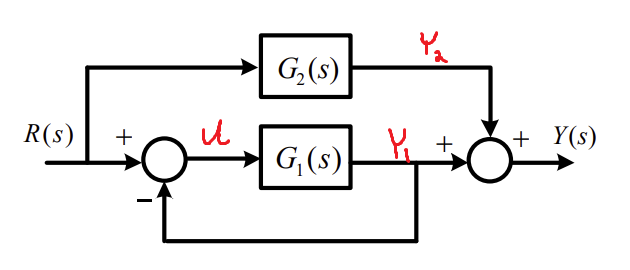
\includegraphics[width=0.99 \linewidth]{transfer.png}
\end{center}

Tracking: Let $L(s) = \frac{L_0(s)}{s^n}$ then it is type $n$ system. Type 0 tracks $r(t) = 1(t) \to \frac{1}{1 + K_p}$,
Type 1 tracks $r(t) = t1(t) \to \frac{1}{K_v}$, and Type 2 tracks $r(t) = \frac{t^2}{2}1(t) \to \frac{1}{K_a}$.
$K = L_0(0)$

PID is $u(t) = k_p (e + \frac{1}{T_1}\int_0^t e(\tau) d\tau + T_D \frac{de}{dt}) \to C(s) = U(s)/E(s) = k_p + \frac{k_p}{T_Is} + k_p T_D s$.

Nyquist: Contour of $L(s)$ as $s$ traverses the RHP. Circle -1 is bad.
gain margin $g_m$ the smalest factor $L$ can be increased before circling -1.
Phase margin $\phi_m$ the largest phase shift $L$ can have before circling -1.
Stability margin $s_m$, shortest distance from the Nyquist plot to $-1$.

Bode: plot $\lg \omega$ vs $20 \lg |G(j\omega)|$. $\omega_{pc}$ is where phase cross 180,
$\omega_{gc}$ is where gain cross 0. $g_m = 1/|G(j\omega_{gc})|$, $\phi_m = 180 + \angle G(j\omega_{pc})$.

Lead compensator: $C(s) = \frac{Ts + 1}{\alpha T s + 1}$, $\phi_{max} = \arcsin \frac{1 - \alpha}{1 + \alpha}$, $\omega_{max} = \frac{1}{T\sqrt{\alpha}}$.
Choose $\omega_{max} = \omega_{gc}$, and $\alpha$ so $\phi_{max} \leq 60\degree$

\section{Time Domain}
controllability: $(A,B)$ is controllable if $C = \begin{bmatrix}
    B & AB & \dots & A^{n-1}B
\end{bmatrix}$ has full row rank.\\
Observability: $(A,C)$ is observable if $O = \begin{bmatrix}
    C \\ CA \\ \vdots \\ CA^{n-1}
\end{bmatrix}$ has full column rank.\\

Pole placement: Compute $C$, and desired $\bar{C}$ (controller realization, negative of desired pole in last row).
$T = \bar{C}C^{-1}$. Compute desired characteristic polynomial: $\Delta(s) = s^n + \bar{a_n}s^{n-1} + \dots + \bar{a_1}$,
then $\bar{F} = \begin{bmatrix}
    \bar{a_1} - a_1 & \dots & \bar{a_n} - a_n \\
\end{bmatrix}$ (from $A$), and finally $F = \bar{F}T$

LQR: $J = \int_0^\infty (x^T Q x + u^T R u) dt$, $Q \succ 0, R \succ 0$. $u = -R^{-1}B^T Px$, $P$ comes from Riccati: $A^T P + PA + Q - PBR^{-1}B^TP = 0$
\section{Other}

Capacitor - $i = C \frac{dv}{dt}$ (state=Voltage), Inductor: $v = L \frac{di}{dt}$ (state=Current), Friction $F = -k v$

\end{document}